\chapter{ARSITEKTUR SISTEM}

Jika membahas arsitektur sistem, maka akan ada beberapa diagram yang terbentuk untuk memudahkan dalam penjelasan sebuah sistem. Penggambaran diagram arsitektur sistem ini berkembang mengikuti model pemrogramannya, dimana dahulu ada yang dikenal dengan \textit{flow-chart} yang menggambarkan alur proses sebuah sistem aplikasi berjalan, mulai dari awal, sampai sistem aplikasi tersebut ditutup dan selesai digunakan, karena memang model pemrograman pada saat ini berbentuk prosedural. 

Namun berkembangnya jaman, dikenal istilah pemrograman berorientasi objek, yang salah satu bahasa pemrogramannya adalah Java. Dengan menggunakan Java, maka diagram \textit{flow-chart} tidak akan bisa melakukan penggambaran alurnya karena pola pada pemrograman berorientasi objek selalu melompat dari satu kelas ke kelas yang lain, dari satu \textit{method} ke \textit{method} yang lain. Maka dibutuhkan penggambaran desain arsitektur yang lain selain \textit{flow-chart}, salah satunya adalah \textit{Unified Modelling Language} (UML).

UML sendiri sebetulnya hanya menggambarkan 2 (dua) sudut pandang dalam pemodelan sistem, yaitu :

\begin{itemize}
  \item \textit{Static view}, yang menekankan pada struktur sistem yang bersifat statis seperti objek, operasi, dan relasi.
  
  \item \textit{Dynamic view}, yang menekankan pada sifat atau tingkah laku dari sistem yang menunjukkan interaksi antar objek didalamnya.
\end{itemize}

\section{Diagram \textit{Use-Case}}

Hal yang pertama digambarkan adalah skenario penggunaan aplikasi secara umum, akan berangkat dari diagram \textit{use-case} seperti pada gambar \ref{fig:uml-use-case} :

\begin{figure}[H]
  \centering
  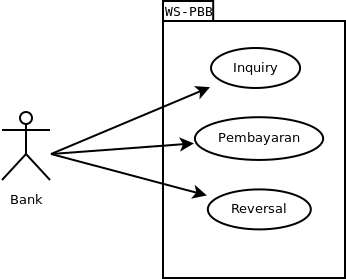
\includegraphics[width=0.5\textwidth]{./resources/uml/uml-use-case}
  \caption{Diagram \textit{use-case}}
  \label{fig:uml-use-case}
\end{figure}

Dari diagram \textit{use-case} diatas, skenarionya adalah bahwa Bank sebagai tempat pembayaran dapat melakukan \textit{request} pada ketiga hal yang disediakan oleh \textit{web services} PBB di DPPK. yaitu :

\begin{itemize}
  \item \textit{Inquiry}
  \item Pembayaran
  \item Reversal
\end{itemize}

Untuk melihat masing-masing proses pada skenario diatas, ada pada diagram \textit{activity} yang dibahas pada bagian selanjutnya. 

\section{Diagram \textit{Activity}}

Diagram \textit{activity} ini akan menunjukan aktivitas yang terjadi untuk setiap skenario pada diagram \textit{use-case}. Berikut skema diagram dari masing-masing skenario yang terbagi menjadi 3 (tiga) diagram berdasarkan jumlah skenario pada diagram \textit{use-case} :

\subsection{Diagram \textit{Activity} Untuk \textit{Inquiry}}

Bagan diagram \textit{activity} untuk \textit{inquiry} ini seperti ditunjukan pada gambar \ref{fig:act-inquiry} :

\begin{figure}[H]
  \centering
  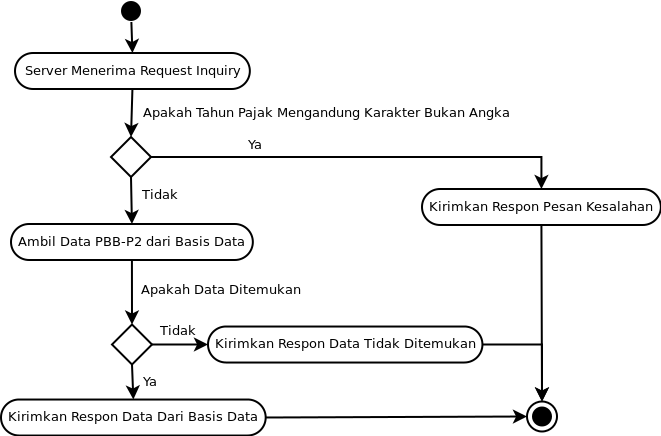
\includegraphics[width=0.8\textwidth]{./resources/uml/uml-act-inquiry}
  \caption{Diagram \textit{Activity} untuk \textit{Inquiry}}
  \label{fig:act-inquiry}
\end{figure}

Aktivitas akan dimulai dari lingkaran penuh di atas, yang kemudian didahului oleh \textit{client} yang melakukan \textit{request} untuk \textit{inquiry} data PBB-P2, hal yang pertama dilakukan adalah melakukan pemeriksaan informasi tahun pajak yang diminta, apakah mengandung karakter atau tidak.

Bila Tahun pajak terisi dengan angka yang wajar, maka aplikasi \textit{web services} akan melakukan koneksi dengan basis data SISMIOP untuk mengambil informasi-informasi yang dibutuhkan oleh \textit{client}.

Bila data tidak ditemukan dalam basis data, maka aplikasi \textit{web services} akan mengirimkan informasi kepada \textit{client} bahwa data yang diminta tidak ditemukan, namun bila data ditemukan, maka disusun dalam format JSON dan dikirimkan ke \textit{client} sebagai respon atas \textit{request} tersebut.

Sampai sini aktivitas selesai.

\subsection{Diagram \textit{Activity} Untuk Pencatatan Pembayaran}

Diagram \textit{activity} untuk melakukan pencatatan pembayaran dapat dilihat seperti pada gambar \ref{fig:act-bayar} :

\begin{figure}[H]
  \centering
  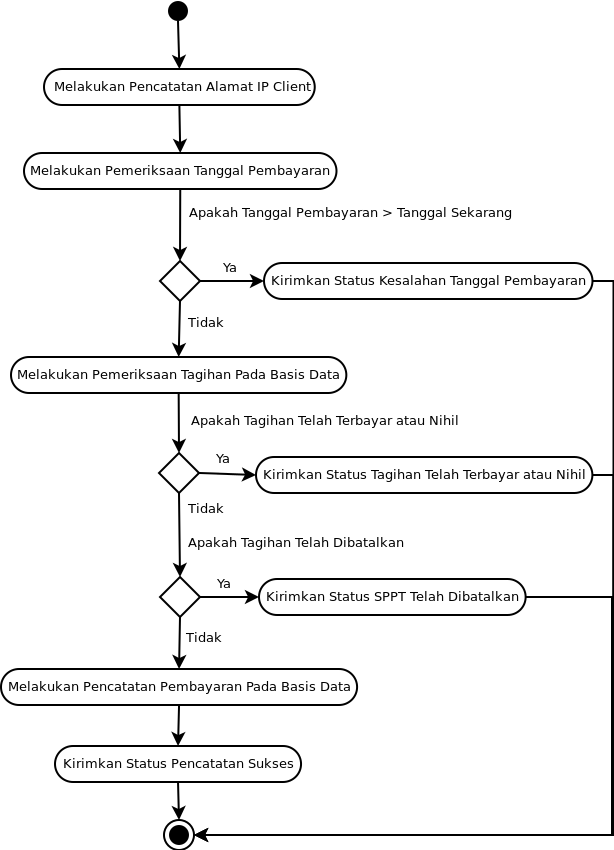
\includegraphics[width=0.8\textwidth]{./resources/uml/uml-act-bayar}
  \caption{Diagram \textit{Activity} Untuk Pencatatan Pembayaran}
  \label{fig:act-bayar}
\end{figure}

Aktivitas pencatatan pembayaran diawali pada saat \textit{client} melakukan \textit{request} pembayaran SPPT PBB-P2, \textit{server web services} akan melakukan pencatatan alamat IP darimana \textit{request} tersebut berasal.

Kemudian \textit{server} akan melakukan pemeriksaan terhadap tanggal pembayaran, apabila tanggal pembayaran melebihi tanggal saat dilakukannya proses pencatatan pembayaran, maka \textit{server} akan mengirimkan status kesalahan tanggal pembayaran ke \textit{client}, dan aktivitas selesai, namun bila tanggal pembayaran kurang dari atau sebelum hari dilakukannya proses pencatatan, maka aktivitas berlanjut ke proses berikutnya.

Pada tahap ini \textit{server} melakukan pemeriksaan tagihan pada basis data, apakah kondisi objek pajak (yang teridentifikasi dari nomor objek pajak) sudah terbayar atau belum, atau tagihannya nihil (tidak ada pajak yang terhutang), bila ya, maka \textit{server} akan mengirimkan status ke \textit{client} bahwa objek yang diminta telah terbayar atau merupakan objek yang piutangnya nihil. bila tidak, maka proses berlanjut.

Proses akhir dari aktivitas ini adalah melakukan pencatatan pembayaran pada basis data, kemudian mengirimkan status bahwa pencatatan tersebut telah selesai. Sampai sini aktivitas telah sampai pada ujung prosesnya.

\subsection{Diagram \textit{Activity} Untuk \textit{Reversal}}

Diagram \textit{activity} untuk melakukan proses \textit{reversal} adalah sebagaimana ditunjukkan pada gambar \ref{fig:act-reversal} :

\begin{figure}[H]
  \centering
  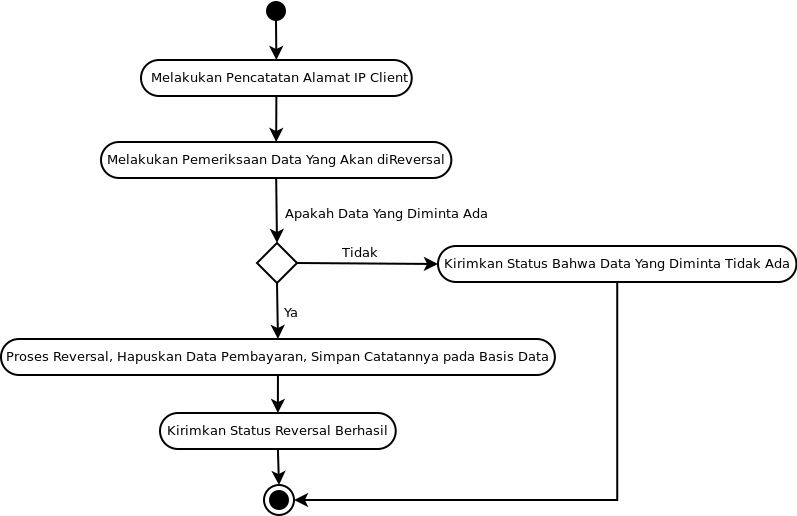
\includegraphics[width=0.8\textwidth]{./resources/uml/uml-act-reversal}
  \caption{Diagram \textit{Activity} Untuk Proses \textit{Reversal}}
  \label{fig:act-reversal}
\end{figure}

Seperti kedua aktivitas sebelumnya, hal yang pertama dilakukan adalah melakukan pencatatan alamat IP dari \textit{client}.

Kemudian melakukan pemeriksan data yang akan direversal, terutama terhadap Nomor Transaksi Pajak Daerah (NTPD) sebagai identitas sebuah transaksi. Apabila data NTPD ini salah, maka \textit{server} akan mengirimkan status kegagalan \textit{reversal} karena data yang diminta tidak ada. Bila data ada, maka melanjutkan ke proses berikutnya.

Langkah berikutnya adalah melakukan pencatatan \textit{request reversal} dan mengirimkan status ke \textit{client} bahwa \textit{reversal} yang diminta telah berhasil dilakukan.

Sampai sini aktivitas \textit{reversal} selesai.

Dari diagram \textit{use-case} dan diagram \textit{activity} telah didapat gambaran umum dari sistem aplikasi yang akan dibangun. Diagram-diagram berikutnya akan lebih detail membahas teknis bagaimana sistem bekerja.

\section{Diagram \textit{Class}}

Pada diagram \textit{class} ini, akan membahas detail dari tiap kelas pembentuk sistem aplikasi \textit{web services} secara keseluruhan. 

\section{Diagram \textit{Sequence}}

\section{Diagram \textit{Statechart}}
